\chapter[Materiales y métodos]{Materiales y métodos}
\label{cp:metodos}
% Extensión estimada: 20--25 páginas.
% Fuentes: sección "Configuración experimental" y subsecciones "Diseño del experimento" del documento de
% experimentación, Propuesta (datasets, técnicas), planes en Codigo/docs/ideas/ (en particular
% split_lesion_semillas_plan_20260912.md). Incorpora el protocolo unificado pedido en el feedback del tutor
% del 12/09/2026 (Codigo/docs/feedback_20260912.md).
%
% Feedback del tutor (14/09/2026):
%  - "Particiones y auditoría de fuga de información" se renombra: el término no se entiende fuera de
%    contexto. Ahora la subsección se llama por lo que produce (la partición disjunta por lesión) y el
%    término "fuga de información (data leakage)" se introduce dentro del texto, definido.
%  - La subsección "Métricas" repetía el marco teórico. Se fusiona con la de selección: el marco teórico
%    define qué es cada métrica, aquí se justifica cuál se usa para decidir.
%  - "Robustez, calibración e interpretabilidad" no decía a qué se refería; se renombra por extenso.
%  - "Sistema propuesto" pasa a llamarse "pipeline", que es el término corriente en el área para la
%    arquitectura completa: clasificador, kNN y generador encadenados.
%  - Se incorpora aquí "Uso de un VLM generativo como clasificador", que estaba en el marco teórico pese a
%    ser parte del enfoque propio.
%
% Revisión 25/09/2026: recibe del marco teórico la prosa ya escrita sobre las categorías de HAM10000
% (§HAM10000), los costos asimétricos de confusión (§selección de métricas) y las partes del reporte
% (§generación de reportes). Ver fichas/02-marco-teorico/historial.md, decisión 14.

% Revisión del tutor del 21/10/2026: orden componentes → integración → evaluación → entorno. La introducción presenta
% primero la lógica metodológica y después, en pocas oraciones, la organización; el pipeline se describe en 3.1.

Este capítulo describe el diseño metodológico con que se responden las preguntas de investigación. El razonamiento
avanza en tres pasos. Primero se fija el problema y se eligen los componentes que pueden abordar cada parte de él por
separado: clasificadores supervisados, modelos visión--lenguaje y generadores de reportes. Después, esos componentes
se integran en un \emph{pipeline} que busca compensar las limitaciones que cada uno tiene por sí solo. Por último, se
definen los criterios y los procedimientos con que se evalúan tanto los componentes como el \emph{pipeline}.

La organización del capítulo sigue ese orden. La Sección~\ref{sec:met_tareas} define las tareas y el flujo de
trabajo, y la Sección~\ref{sec:met_datasets} presenta los conjuntos de datos. Las Secciones~\ref{sec:met_supervisados}
a~\ref{sec:met_generacion} describen los componentes, y la Sección~\ref{sec:met_pipeline} los integra. La evaluación
ocupa las Secciones~\ref{sec:met_protocolo} y~\ref{sec:met_complementarios}. Por último, la
Sección~\ref{sec:met_diseno} ordena los experimentos por etapas, y la Sección~\ref{sec:met_entorno} reúne el entorno
experimental.

\section{Definición de las tareas}
\label{sec:met_tareas}

El clasificador asigna cada imagen a una etiqueta de un inventario cerrado, y ese inventario es el de
HAM10000, con siete categorías: \gls{mel}, \gls{nv}, \gls{bcc}, \gls{akiec}, \gls{bkl}, \gls{df} y
\gls{vasc}. Según su gravedad, NV, BKL, DF y VASC son benignas, AKIEC reúne lesiones premalignas y
carcinomas in situ, y MEL y BCC son malignas~\cite{tschandl2018ham10000}. Esa gradación determina
cuánto cuesta cada confusión del clasificador, y con ello qué métricas se usan para juzgarlo
(Sección~\ref{sec:met_seleccion}).

El reporte dermatológico deja por escrito la lectura de la lesión, y de sus partes el trabajo se ocupa
de dos: la descripción de lo que se ve y la impresión diagnóstica. Son las que corresponden a las dos
tareas del problema, y las que los conjuntos de pares imagen--texto del área anotan junto a cada
imagen~\cite{shen2025skincare}. El diagnóstico diferencial y la recomendación de manejo, que un reporte
clínico completo también lleva, quedan fuera del alcance.

\pendiente{Definición formal de las tres tareas (clasificación en siete clases, detección binaria de
melanoma, generación del reporte), con su entrada, su salida y la restricción de cómputo.}

% Extensión estimada: 4.5--5 páginas (catorce párrafos, dos tablas, tres figuras y un fragmento de texto).
% Fuentes: conteos propios sobre Codigo/data/raw/HAM10000/HAM10000_metadata, Codigo/data/splits/ham10000_splits.json
% y ham10000_splits_lesion.json (solo lectura, 2026-10-11); Codigo/outputs/results/leakage_analysis.json;
% Codigo/scripts/make_lesion_disjoint_split.py; Codigo/scripts/prepare_data.py (splits de SkinCaRe);
% Codigo/data/splits/mmskin_splits.json, hiba_splits.json, skincare_*_splits.json. Figuras de HAM10000 generadas con
% Codigo/scripts/plot_ham_dataset_figs.py. Papers en Papers/derma/ (SkinCaRe, MM-Skin, HIBA, Derm1M).
% Claves: tschandl2018ham10000, shen2025skincare, groh2021neural, daneshjou2022disparities, daneshjou2022skincon,
% zeng2025mmskin, riccilara2023dataset, yan2025derm1miccv.
% Revisión del autor del 18/10/2026: menos cifras en el texto; los conteos completos quedan en tablas y figuras.
\section{Conjuntos de datos}
\label{sec:met_datasets}

El trabajo usa cinco conjuntos de datos de dermatología, que se diferencian por la modalidad de sus imágenes y por
el tipo de anotación que acompaña a cada una. \emph{HAM10000} reúne imágenes dermatoscópicas con un diagnóstico
confirmado y sin texto. \emph{SkinCaRe} y \emph{MM-Skin}, en cambio, asocian cada imagen a un texto clínico escrito
por dermatólogos, por un modelo de lenguaje o tomado de libros de dermatología. \emph{HIBA} aporta imágenes
dermatoscópicas y clínicas de un hospital argentino, y \emph{Derm1M} es un corpus de más de un millón de pares
imagen--texto. La Tabla~\ref{tab:met_conjuntos} resume, para cada uno, la modalidad, el tamaño, el uso en el trabajo y
el origen del texto de referencia.

Cada conjunto cumple un papel distinto en la experimentación, según sirva para entrenar, para evaluar o solo de forma
indirecta. \emph{HAM10000} es el único etiquetado con las siete categorías de la tarea, de modo que con él se entrenan
los clasificadores, se eligen sus configuraciones en validación y se evalúan en prueba todos los modelos de
clasificación y el \emph{pipeline}. Por esa razón es el conjunto central del trabajo, y sus propiedades, que se
analizan a continuación, determinan cómo se parte y con qué métricas se evalúa. \emph{SkinCaRe}, en cambio, se usa
para entrenar a los generadores de reportes, y \emph{MM-Skin}, para evaluarlos contra un texto de referencia.
\emph{HIBA} se usa solo como prueba externa, para comprobar si los clasificadores mantienen su desempeño en otra
población. Por último, \emph{Derm1M} no se usa de forma directa: es el conjunto con el que sus autores preentrenaron
DermLIP, uno de los modelos de la Sección~\ref{sec:met_clasif_vlm}.

\begin{table}[H]
    \centering
    \small
    \caption{Conjuntos de datos: modalidad, tamaño, uso en el trabajo y origen del texto de referencia.}
    \label{tab:met_conjuntos}
    \begin{tabularx}{\textwidth}{@{}>{\raggedright\arraybackslash}p{1.8cm}
        >{\raggedright\arraybackslash}p{2.5cm} >{\raggedright\arraybackslash}p{2.2cm}
        >{\raggedright\arraybackslash\hspace{0pt}}p{2.4cm} >{\raggedright\arraybackslash\hspace{0pt}}X@{}}
        \toprule
        \textbf{Conjunto} & \textbf{Modalidad} & \textbf{Tamaño} & \textbf{Uso} & \textbf{Origen del texto de referencia} \\
        \midrule
        \emph{HAM10000} & Dermatoscópica & 10\,015 imágenes; 7\,470 lesiones
            & Clasificación (entrenamiento, validación y prueba)
            & Sin texto; etiqueta confirmada por histopatología, seguimiento, consenso o microscopía confocal \\
        \filasep
        \emph{SkinCAP} (\emph{SkinCaRe}) & Clínica (fotografía) & 3\,561 imágenes
            & Entrenamiento de los generadores
            & Descripciones de cuatro dermatólogos, escritas en chino y traducidas al inglés \\
        \filasep
        \emph{SkinCoT} (\emph{SkinCaRe}) & Clínica (fotografía) & 3\,041 imágenes
            & Entrenamiento de los generadores; su prueba, evaluación con referencia
            & Razonamiento escrito por un modelo de lenguaje con la etiqueta a la vista y revisado por dermatólogos \\
        \filasep
        \emph{MM-Skin} & Clínica, dermatoscópica y patológica
            & 11\,039 imágenes; 9\,369 pares imagen--texto
            & Evaluación de los generadores con referencia
            & Descripciones de libros de texto de dermatología \\
        \filasep
        \emph{HIBA} & Dermatoscópica y clínica
            & 1\,616 imágenes; 1\,246 lesiones
            & Evaluación externa de los clasificadores (solo prueba)
            & Diagnóstico de dermatólogos del hospital, con histopatología en las lesiones extirpadas \\
        \filasep
        \emph{Derm1M} & Dermatoscópica y clínica & 1\,029\,761 pares imagen--texto
            & Preentrenamiento de DermLIP por sus autores (no se usa de forma directa)
            & Fuentes web, educativas y bases públicas; texto procesado con un \gls{llm} \\
        \bottomrule
    \end{tabularx}
\end{table}

\subsection{HAM10000: composición y análisis exploratorio}
\label{sec:met_ham}

\emph{HAM10000} contiene 10\,015 imágenes dermatoscópicas tomadas en Viena y en
Queensland~\cite{tschandl2018ham10000}, que según sus metadatos corresponden a 7\,470 lesiones. El conjunto no identifica a los pacientes, así que la lesión es la agrupación
más fina disponible. Tres de sus propiedades condicionan cómo se entrena y se evalúa un clasificador: cómo se reparten
las clases, cuántas imágenes tiene cada lesión y con qué respaldo se asignó cada etiqueta.

En primer lugar, la distribución de las clases es muy desigual (Figura~\ref{fig:met_ham_dist}). \gls{nv} reúne dos tercios de las
imágenes, mientras que \gls{df} y \gls{vasc} no llegan al 1.5\,\% cada una. Un clasificador que respondiera siempre NV
acertaría dos de cada tres imágenes sin reconocer ninguna otra clase, de modo que la exactitud global no sirve para
distinguir entre modelos. Esta es la razón por la que el trabajo usa métricas que dan a todas las clases el mismo peso
(Sección~\ref{sec:met_protocolo}).

\begin{figure}[H]
    \centering
    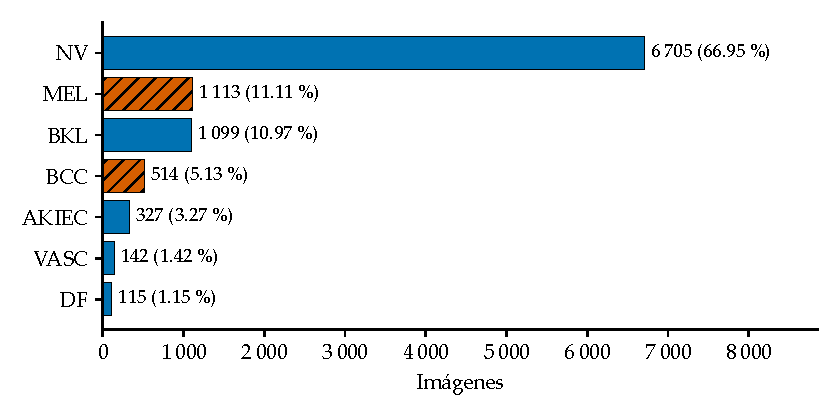
\includegraphics[width=0.8\textwidth]{Figures/Capitulos/03-Materiales-Metodos/ham-distribucion.pdf}
    \caption{Imágenes por clase en \emph{HAM10000} y su porcentaje sobre el total. MEL y BCC en bermellón con trama; las demás clases en azul.}
    \label{fig:met_ham_dist}
\end{figure}

La segunda propiedad afecta a la partición. Una misma lesión puede tener hasta seis imágenes, y las 1\,956 lesiones
con más de una reúnen el 45\,\% del conjunto (Figura~\ref{fig:met_ham_lesiones}). Una situación a evitar es que
imágenes de una misma lesión caigan en entrenamiento y en prueba, ya que el modelo puede reconocer la lesión en lugar
de generalizar a lesiones nuevas, y la prueba deja de medir lo que dice medir. Por eso la partición tiene que agrupar
las imágenes de cada lesión.

\begin{figure}[H]
    \centering
    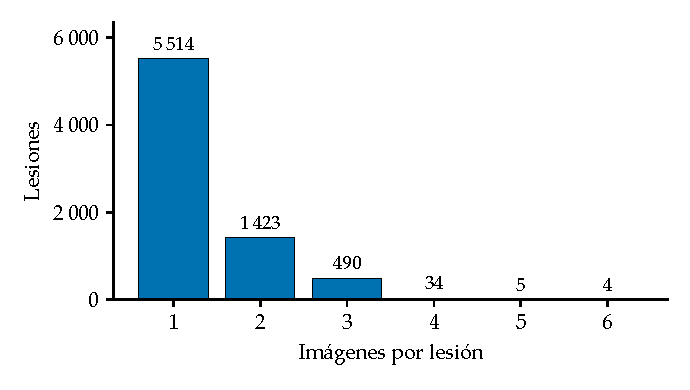
\includegraphics[width=0.7\textwidth]{Figures/Capitulos/03-Materiales-Metodos/ham-imagenes-por-lesion.pdf}
    \caption{Lesiones de \emph{HAM10000} según el número de imágenes que tienen, de una a seis.}
    \label{fig:met_ham_lesiones}
\end{figure}

La tercera propiedad es el respaldo de las etiquetas, que no es el mismo en todas las clases. La histopatología
confirma algo más de la mitad de las imágenes, y todas las de MEL, BCC y AKIEC. En cambio, casi dos tercios de las NV
se confirmaron por seguimiento clínico o por consenso de los autores. La referencia es, por lo tanto, más sólida en
las clases malignas y premalignas que en las benignas. Como ilustración, la Figura~\ref{fig:met_ham_ejemplos} muestra
una imagen de cada clase.

\begin{figure}[H]
    \centering
    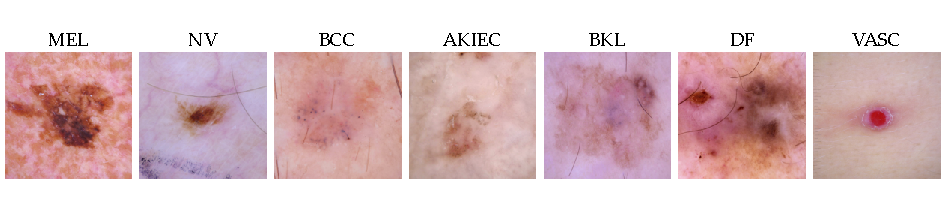
\includegraphics[width=\textwidth]{Figures/Capitulos/03-Materiales-Metodos/ham-ejemplos.pdf}
    \caption{Una imagen dermatoscópica por clase, la primera confirmada por histopatología de cada una. Imágenes de \emph{HAM10000}~\cite{tschandl2018ham10000}, licencia CC BY-NC 4.0. El orden es MEL, NV, BCC, AKIEC, BKL, DF y VASC, las siglas del conjunto.}
    \label{fig:met_ham_ejemplos}
\end{figure}

\subsection{Partición disjunta por lesión}
\label{sec:met_particiones}

La forma habitual de partir un conjunto es asignar cada imagen al azar a una partición, manteniendo en cada una la
proporción de las clases. Con ese procedimiento, una partición frecuente destina el 70\,\% de las imágenes a
entrenamiento, el 15\,\% a validación y el 15\,\% a prueba, y así está construida la partición original de
\emph{HAM10000} con la que comenzó este trabajo. Sin embargo, como la asignación se hace imagen por imagen, dos
imágenes de una misma lesión pueden quedar en particiones distintas. En la partición original, 36 de cada 100
imágenes de prueba tienen otra imagen de su misma lesión en entrenamiento, y entre los melanomas la proporción es de
63 de cada 100.

Esta coincidencia es una fuga de información entre particiones (\emph{data leakage};
Sección~\ref{sec:marco_regularizacion}): el modelo pudo ver en el entrenamiento la misma lesión que se le pide
clasificar, de modo que la prueba ya no mide el desempeño sobre lesiones nuevas. Además, la fuga no afecta a todas las
clases por igual. En NV alcanza al 27\,\% de las imágenes de prueba, mientras que en BCC llega al 70\,\%, así que las
dos clases malignas, que son las que más importan, son las más afectadas.

Para eliminar la fuga, la partición nueva conserva completa la prueba original, de modo que los resultados de los
\glspl{vlm} y del \emph{pipeline}, medidos sobre ella, siguen siendo comparables. Del entrenamiento y la validación
originales se descartan las 776 imágenes cuya lesión aparece en la prueba, y las restantes se reparten con
\texttt{StratifiedGroupKFold} de scikit-learn, con la lesión como grupo, el diagnóstico como estrato y la semilla 42.
Con este procedimiento se obtienen 6\,447 imágenes de entrenamiento y 1\,289 de validación, sin lesiones compartidas entre particiones
(Tabla~\ref{tab:met_tamanos}). El costo es que el entrenamiento tiene un 8\,\% menos de imágenes que el de la partición
original (6\,447 frente a 7\,010). Además, en validación DF y VASC quedan con menos de 20 imágenes, así que sus métricas
por clase en ese conjunto cambian mucho con pocos aciertos.

\begin{table}[H]
    \centering
    \caption{Imágenes por clase y partición de \emph{HAM10000}.}
    \label{tab:met_tamanos}
    \begin{tabularx}{\textwidth}{@{}>{\raggedright\arraybackslash}X r r r r@{}}
        \toprule
        \textbf{Clase} & \textbf{Entrenamiento} & \textbf{Validación} & \textbf{Prueba} & \textbf{Descartadas} \\
        \midrule
        AKIEC & 207 & 41 & 49 & 30 \\
        BCC & 307 & 62 & 77 & 68 \\
        BKL & 682 & 137 & 165 & 115 \\
        DF & 73 & 14 & 17 & 11 \\
        MEL & 661 & 132 & 167 & 153 \\
        NV & 4\,427 & 885 & 1\,006 & 387 \\
        VASC & 90 & 18 & 22 & 12 \\
        \midrule
        \textbf{Total} & \textbf{6\,447} & \textbf{1\,289} & \textbf{1\,503} & \textbf{776} \\
        \bottomrule
    \end{tabularx}
\end{table}

Además de corregirla, interesa saber cuánto sobreestimaba la fuga el desempeño de los clasificadores. Para estimarlo,
el Capítulo~\ref{cp:res_clasif} compara el resultado sobre la prueba completa con el que se obtiene sobre sus 894
imágenes cuya lesión no aparecía ni en entrenamiento ni en validación de la partición original. Como control se usa
DermLIP sin ajuste, que no vio \emph{HAM10000}: si su desempeño también cambia entre ambos conjuntos, el cambio se debe
a la composición del subconjunto y no a la fuga. A diferencia de \emph{HAM10000}, los demás conjuntos no pasan por esta
partición, porque cada uno trae su propia división o se usa completo como prueba.

\subsection{SkinCaRe: SkinCAP y SkinCoT}

En cuanto a la generación de texto, \emph{SkinCaRe} reúne los pares imagen--texto con que se entrenan los generadores
de reportes (Sección~\ref{sec:met_generacion}). Está formado por dos subconjuntos con textos de distinto tipo:
\emph{SkinCAP}, con descripciones escritas por dermatólogos, y \emph{SkinCoT}, con razonamientos diagnósticos.
\emph{SkinCAP} tiene 4\,000 imágenes clínicas tomadas de
\emph{Fitzpatrick 17k} y de \emph{DDI}~\cite{groh2021neural,daneshjou2022disparities}, con descripciones que
escribieron cuatro dermatólogos en chino y que luego se tradujeron al inglés y se revisaron~\cite{shen2025skincare}.
De ellas se excluyen 439 que llevan la marca de descarte que \emph{SKINCON} daba a sus anotadores
para las imágenes de mala calidad~\cite{daneshjou2022skincon}, y las 3\,561 restantes se reparten por imagen con las
mismas proporciones de 70, 15 y 15\,\%.

Por su parte, \emph{SkinCoT} aporta 3\,041 imágenes clínicas del atlas DermNet con un razonamiento diagnóstico escrito para cada
una~\cite{shen2025skincare}. El texto lo produce un modelo de lenguaje que recibe la etiqueta verdadera, y
dermatólogos lo revisan y descartan los de menor puntaje. Como se escribió conociendo el diagnóstico, el razonamiento
muestra cómo se justifica una etiqueta conocida y no cómo se llega a ella desde la imagen, una limitación que pesa al
leer los resultados de generación. Además, el formato intercala bloques \texttt{\textless{}think\textgreater{}} entre
las oraciones y termina con el diagnóstico. Para ilustrarlo, el fragmento siguiente, de un caso de párpados, muestra la
forma; la traducción es propia.

\begin{quote}
    \small
    \texttt{\textless{}think\textgreater{}} First, I observe the primary location: the changes are specifically affecting
    the eyelids (both upper and lower). The skin here is thin and sensitive, making it prone to certain dermatological
    conditions. \texttt{\textless{}/think\textgreater{}}

    \noindent Traducción propia: «Primero, observo la localización principal: los cambios afectan específicamente los
    párpados (superior e inferior). La piel aquí es fina y sensible, lo que la hace propensa a ciertas afecciones
    dermatológicas.»
\end{quote}

\subsection{MM-Skin, HIBA y Derm1M}

A diferencia de \emph{SkinCaRe}, que se usa para entrenar, \emph{MM-Skin} es el conjunto con que se evalúa la
generación contra un texto de referencia. Sus textos son descripciones de quince libros de texto de dermatología,
asociadas a imágenes clínicas, dermatoscópicas y patológicas~\cite{zeng2025mmskin}, y las métricas con referencia se
calculan sobre su partición de prueba (Sección~\ref{sec:met_eval_generacion}). Ninguno de los generadores ajustados en
este trabajo vio \emph{MM-Skin}.
SkinVL, en cambio, sí se ajustó con él y por ello no se evalúa sobre este conjunto.

Por otra parte, \emph{HIBA} reúne 1\,616 imágenes de 623 pacientes de un hospital de Buenos Aires, con licencia CC
BY~\cite{riccilara2023dataset}. Es el único conjunto de otra población y se usa completo como prueba externa, de modo que
ningún modelo se entrena con él (Sección~\ref{sec:marco_generalizacion}). Además, cuatro de cada cinco imágenes son
dermatoscópicas y el resto clínicas, y el melanoma tiene más peso que en \emph{HAM10000} (16\,\% frente a 11\,\%).
Para usarlo con los clasificadores, sus diagnósticos se llevan a las siete categorías de \emph{HAM10000}. En ese
mapeo, el carcinoma escamoso pasa a AKIEC, una aproximación que agrega ruido a la comparación y que se retoma en la
Sección~\ref{sec:met_complementarios}.

Por último, \emph{Derm1M} es el corpus de 1\,029\,761 pares imagen--texto con el que se preentrenó DermLIP~\cite{yan2025derm1miccv}.
Sus imágenes provienen de videos, artículos científicos, foros médicos, conjuntos públicos y material educativo, y sus
textos se limpiaron y resumieron con un \gls{llm}. Entre las fuentes declaradas no figura \emph{HAM10000}, aunque no
puede descartarse que alguna publicación reproduzca imágenes de ese conjunto. El trabajo usa los pesos publicados de
DermLIP sin reentrenarlo, así que \emph{Derm1M} no se usa para entrenar ni para evaluar.

Las características de estos conjuntos orientan la elección de los modelos que se presentan a continuación. Con unas
6\,400 imágenes etiquetadas para siete clases, entrenar un clasificador desde cero no es viable, y por eso los
clasificadores supervisados parten de pesos preentrenados. Por la misma razón, la clasificación con \glspl{vlm} incluye
a DermLIP, que llega preentrenado sobre imágenes de dermatología. Por otra parte, como los textos clínicos disponibles
no usan las siete categorías de \emph{HAM10000}, los generadores aprenden a redactar con \emph{SkinCaRe} y reciben el
diagnóstico de un clasificador, como se describe en la Sección~\ref{sec:met_pipeline}.

\section{Clasificadores supervisados}
\label{sec:met_supervisados}
% Extensión estimada: 4--4.5 páginas, con una figura y tres tablas, en tres subsecciones.
% Fuentes: src/models/classifiers.py; src/data/transforms.py; src/training/recipes.py, optim_groups.py,
% schedulers.py, losses.py; src/evaluation/tta.py; scripts/train_classifier.py; scripts/toko/submit_sweep.py
% y submit.py (valores efectivos); scripts/sweep_utils.py y configs/sweeps/phase1_modern_sweep_grid.yaml
% (grilla); logs de entrenamiento (parámetros); docs/resul/split_lesion_resul_20260926.md (ganadores, semillas,
% réplica del desbalance); docs/resul/densenet_vit_moderna_resul_20261017.md (DenseNet121 y ViT-B/16 con la
% configuración de su familia, tres semillas); scripts/lesion_split_report.py, classifier_ensemble.py,
% melanoma_detection.py. No se usan como fuente los configs/*.yaml de clasificación, porque train_classifier.py no los lee.
% Revisión del autor del 18/10/2026: solo la configuración final; sin comparar recetas ni describir la búsqueda
% anterior de DenseNet121 y ViT-B/16, cuyas corridas quedan fuera del capítulo.
% Revisión del tutor del 21/10/2026: estructura común con 3.4 (propósito → modelos seleccionados → configuración →
% procedimiento experimental); el motivo de la elección antes de las características; figura de uso; los criterios
% de selección se definen en 3.7 y acá solo se nombran.

Los clasificadores supervisados cumplen dos funciones en el trabajo. Por un lado, resuelven la clasificación (T1) y la
detección de melanoma (T2) con modelos entrenados solo con imágenes, y son la línea base
(Sección~\ref{sec:marco_swin}) con la que se mide si un \gls{vlm} clasifica igual de bien. Por otro lado, dentro del
\emph{pipeline}, son los que fijan el diagnóstico que recibe el generador. Para cumplir ambas funciones hacen falta
modelos que aprendan de unas 6\,400 imágenes y que puedan entrenarse en una GPU de consumo.

\subsection{Modelos seleccionados}
\label{sec:met_supervisados_arquitecturas}

Las dos familias de arquitecturas de visión, las convolucionales y las basadas en transformers, parten de supuestos
distintos sobre la imagen, y ninguna se impone de antemano (Sección~\ref{sec:marco_vision}). A su vez, los trabajos de
clasificación dermatológica revisados evalúan casi solo redes convolucionales (Sección~\ref{sec:estado_arte_diagnostico}).
Por ello, el trabajo compara las dos familias con el mismo procedimiento, y de cada una toma dos de los modelos
presentados en el Capítulo~\ref{cp:marco}: DenseNet121 y ConvNeXt-Tiny entre las convolucionales, y ViT-B/16 y
Swin-Tiny entre las basadas en transformers. Las variantes Tiny, con unos 27.5 millones de parámetros, tienen un tercio
de los de ViT-B/16 (Tabla~\ref{tab:met_modelos_sup}).

Los cuatro modelos se usan de la misma manera, que muestra la Figura~\ref{fig:met_clasificador}. Cada uno parte de
pesos preentrenados en \emph{ImageNet}-1K, y su última capa se reemplaza por una cabeza de siete salidas, precedida
por un \emph{dropout} de 0.3. La softmax convierte esas salidas en una probabilidad por clase, de la que se obtienen
las dos respuestas del clasificador: la clase de mayor probabilidad, para T1, y la probabilidad de melanoma, que se
compara con un umbral para T2.

% Figura: uso de un clasificador supervisado en este trabajo, fig:met_clasificador. Usada en sec:met_supervisados (3.3).
% No redibuja la arquitectura (Cap. 2): muestra entrada, red preentrenada, cabeza nueva, salidas para T1 y T2 y qué se
% entrena en cada etapa. Revisión del tutor del 21/10/2026 (figuras de los modelos). Ancho: unos 148 mm.

\begin{figure}[H]
    \centering
    \hyphenpenalty=10000 \exhyphenpenalty=10000
    \begin{tikzpicture}[x=1mm, y=1mm]

        \node[figentrada, text width=15mm] (img) at (9, 0) {imagen\\{\footnotesize $224 \times 224$}};
        \node[figtarea, text width=32mm] (red) at (42, 0)
            {red preentrenada\\{\footnotesize DenseNet121, ConvNeXt-Tiny, ViT-B/16 o Swin-Tiny}};
        \node[figtarea, text width=21mm] (cab) at (79, 0) {cabeza nueva\\{\footnotesize \emph{dropout} y lineal de 7 salidas}};
        \node[fignodo, text width=17mm, fill=figrelleno] (sm) at (105, 0) {softmax\\{\footnotesize $p_c$ por clase}};
        \node[figsalida, text width=21mm] (t1) at (135, 9) {T1: clase de mayor $p_c$};
        \node[figsalida, text width=21mm] (t2) at (135, -9) {T2: $p_{\text{MEL}}$ frente a un umbral};

        \draw[figflecha] (img) -- (red);
        \draw[figflecha] (red) -- (cab);
        \draw[figflecha] (cab) -- (sm);
        \draw[figflecha] (sm.east) -- ++(4, 0) |- (t1.west);
        \draw[figflecha] (sm.east) -- ++(4, 0) |- (t2.west);

        \node[figetiqueta, align=center, text=fignaranja!70!black, anchor=north] at ([yshift=-2mm]red.south)
            {etapa 1: congelada\\etapa 2: se ajusta toda};
        \node[figetiqueta, align=center, text=fignaranja!70!black, anchor=north] at ([yshift=-2mm]cab.south)
            {se entrena en\\las dos etapas};
        \node[figetiqueta, anchor=south] at ([yshift=2mm]red.north) {pesos de \emph{ImageNet}-1K};

    \end{tikzpicture}
    \caption{Uso de los clasificadores supervisados: la red preentrenada recibe una cabeza nueva, y la probabilidad por
    clase resuelve T1 y T2.}
    \label{fig:met_clasificador}
\end{figure}


\begin{table}[H]
    \centering
    \caption{Los cuatro clasificadores: familia, preentrenamiento, cabeza, parámetros con cabeza de siete clases y tamaño de lote.}
    \label{tab:met_modelos_sup}
    \small
    \begin{tabularx}{\textwidth}{@{}>{\raggedright\arraybackslash}p{2.1cm}>{\raggedright\arraybackslash}X>{\raggedright\arraybackslash}p{1.9cm}>{\raggedright\arraybackslash}p{2.6cm}>{\raggedleft\arraybackslash}p{1.85cm}>{\raggedleft\arraybackslash}p{0.8cm}@{}}
        \toprule
        \textbf{Modelo} & \textbf{Familia} & \textbf{Pesos iniciales} & \textbf{Cabeza} & \textbf{Parámetros} & \textbf{Lote} \\
        \midrule
        DenseNet121 & Red convolucional, bloques densos & \emph{ImageNet}-1K & \emph{Dropout} 0.3 y lineal de 7 salidas & 6\,961\,031 & 32 \\
        \filasep
        ConvNeXt-Tiny & Red convolucional moderna & \emph{ImageNet}-1K & \emph{Dropout} 0.3 y lineal de 7 salidas & 27\,825\,511 & 32 \\
        \filasep
        ViT-B/16 & Transformer visual, parches de $16 \times 16$ & \emph{ImageNet}-1K & \emph{Dropout} 0.3 y lineal de 7 salidas & 85\,804\,039 & 16 \\
        \filasep
        Swin-Tiny & Transformer jerárquico, con ventanas & \emph{ImageNet}-1K & \emph{Dropout} 0.3 y lineal de 7 salidas & 27\,524\,737 & 16 \\
        \bottomrule
    \end{tabularx}
\end{table}

\subsection{Configuración del entrenamiento}
\label{sec:met_supervisados_receta}

La configuración parte de la entrada. Las imágenes de \emph{HAM10000} se reducen una sola vez a $224 \times 224$
píxeles, sin conservar su proporción, y todos los modelos de este capítulo parten de esa versión. Los clasificadores,
además, las reciben normalizadas con la media y el desvío de \emph{ImageNet}. Como el entrenamiento cuenta con 6\,447
imágenes (Sección~\ref{sec:met_particiones}), el riesgo principal es el sobreajuste
(Sección~\ref{sec:marco_regularizacion}). Para reducirlo se aplican aumentos de datos que cambian la imagen sin
cambiar su clase, ya que una misma lesión puede fotografiarse con otro encuadre, otra orientación u otra iluminación.
En concreto, se toma un recorte aleatorio de entre el 70\,\% y el 100\,\% del área, se voltea la imagen horizontalmente
con probabilidad 0.5, se aplican dos transformaciones de RandAugment~\cite{cubuk2020randaugment} con una magnitud $M$
que se elige por búsqueda, y se borra un rectángulo al azar con probabilidad 0.25~\cite{zhong2020random}.

En validación y en prueba, en cambio, no hay aumento. La imagen se redimensiona a $256 \times 256$ y se recorta el
centro de $224 \times 224$. Las probabilidades finales de ambas particiones se obtienen con \gls{tta}
(Sección~\ref{sec:marco_regularizacion}), que promedia las de la imagen y su reflejo horizontal, mientras que la
validación de cada época usa una sola vista.

Con las entradas fijadas, cada modelo se adapta a \emph{HAM10000} en dos etapas, que corresponden a las dos opciones
de la Sección~\ref{sec:marco_transferencia}: primero la extracción de características y después el ajuste fino. En la
primera etapa, con el resto de la red congelado, se entrena solo la cabeza nueva durante una época, de modo que el
ajuste fino no parta de una cabeza inicializada al azar. En la segunda se descongela toda la red, y cada capa recibe
0.85 veces la tasa de aprendizaje de la capa siguiente (Ecuación~\ref{eq:marco_llrd}). Esta etapa dura hasta 39
épocas, con tres de calentamiento lineal y decaimiento coseno de la tasa~\cite{goyal2017accurate,loshchilov2017sgdr}.

Los demás elementos del entrenamiento son comunes a los cuatro modelos. El optimizador es
AdamW~\cite{loshchilov2019decoupled}, y la función de pérdida es la entropía cruzada con suavizado de etiquetas de
0.1~\cite{szegedy2016rethinking,muller2019does}. Finalmente, la detención temprana corta el entrenamiento si el F1
ponderado de validación no mejora en cinco épocas, y se conserva la mejor época; la
Sección~\ref{sec:met_seleccion} justifica ese criterio. La Tabla~\ref{tab:met_receta} reúne estos valores.

\begin{table}[H]
    \centering
    \caption{Parámetros de entrenamiento comunes a los cuatro clasificadores.}
    \label{tab:met_receta}
    \small
    \begin{tabularx}{\textwidth}{@{}>{\raggedright\arraybackslash}p{4.2cm}>{\raggedright\arraybackslash}X@{}}
        \toprule
        \textbf{Parámetro} & \textbf{Valor} \\
        \midrule
        Optimizador & AdamW \\
        \filasep
        Épocas & Hasta 40: una de cabeza y hasta 39 de red completa \\
        \filasep
        Decaimiento de la tasa por capa & 0.85 \\
        \filasep
        Planificador & Calentamiento lineal de tres épocas desde 0.1 de la tasa; luego coseno \\
        \filasep
        Función de pérdida & Entropía cruzada, con suavizado de etiquetas de 0.1 \\
        \filasep
        Detención temprana & Paciencia de cinco épocas sobre el F1 ponderado de validación \\
        \filasep
        Aumento de datos & Recorte aleatorio (70--100\,\% del área), volteo horizontal, RandAugment ($N = 2$) y borrado aleatorio ($p = 0.25$) \\
        \filasep
        Inferencia & \gls{tta} con la imagen y su reflejo horizontal \\
        \filasep
        Precisión numérica & \emph{bfloat16} (bf16) \\
        \bottomrule
    \end{tabularx}
\end{table}

\subsection{Procedimiento experimental}
\label{sec:met_supervisados_ensamble}

Además de los valores comunes, tres hiperparámetros se eligen por búsqueda: la tasa de aprendizaje, el decaimiento de
pesos y la magnitud de RandAugment (Tabla~\ref{tab:met_barrido}). Las cinco tasas se cruzan con los tres
decaimientos, y cada magnitud se asigna a cinco de esas 15 combinaciones. Cada combinación se entrena con y sin pesos
por clase en la función de pérdida (Sección~\ref{sec:marco_desbalance}), lo que suma 30 configuraciones por modelo,
con una ejecución cada una. La búsqueda se hizo sobre Swin-Tiny y ConvNeXt-Tiny, y en ambos ganó, con el criterio de la
Sección~\ref{sec:met_seleccion}, una configuración sin pesos por clase. DenseNet121 y ViT-B/16, en cambio, usan la
configuración ganadora del modelo de su misma familia: la de ConvNeXt-Tiny en el caso de DenseNet121 y la de Swin-Tiny
en el de ViT-B/16. Así los cuatro se comparan con el mismo procedimiento, aunque si DenseNet121 o ViT-B/16 rinden
menos, puede deberse a que la configuración heredada no es la mejor para ellos.

\begin{table}[H]
    \centering
    \caption{Hiperparámetros explorados en la búsqueda y valores elegidos. DenseNet121 usa los de ConvNeXt-Tiny, y ViT-B/16, los de Swin-Tiny.}
    \label{tab:met_barrido}
    \small
    \begin{tabularx}{\textwidth}{@{}>{\raggedright\arraybackslash}p{3.4cm}>{\raggedright\arraybackslash}X>{\raggedright\arraybackslash}p{2.0cm}>{\raggedright\arraybackslash}p{2.2cm}@{}}
        \toprule
        \textbf{Parámetro} & \textbf{Valores explorados} & \textbf{Swin-Tiny} & \textbf{ConvNeXt-Tiny} \\
        \midrule
        Tasa de aprendizaje & $3.0 \times 10^{-5}$; $7.5 \times 10^{-5}$; $1.5 \times 10^{-4}$; $2.5 \times 10^{-4}$; $5.0 \times 10^{-4}$ & $7.5 \times 10^{-5}$ & $3.0 \times 10^{-5}$ \\
        \filasep
        Decaimiento de pesos & 0.01; 0.05; 0.10 & 0.10 & 0.05 \\
        \filasep
        Magnitud de RandAugment ($M$) & 6; 9; 12, cada valor en cinco de las 15 combinaciones & 6 & 9 \\
        \filasep
        Pesos por clase & Inversos a la frecuencia; ninguno & Ninguno & Ninguno \\
        \bottomrule
    \end{tabularx}
\end{table}

Una vez elegida la configuración, cada modelo se entrena tres veces, con distinta inicialización aleatoria, porque las
métricas de las clases minoritarias dependen de pocas imágenes y una sola ejecución no muestra cuánto varía el
resultado.

Los pesos por clase no son la única forma de abordar el desbalance (Sección~\ref{sec:marco_desbalance}), y por eso se
comparan aparte cuatro funciones de pérdida sobre Swin-Tiny, ConvNeXt-Tiny y DenseNet121:
\begin{itemize}
    \item \textbf{Entropía cruzada sin pesos}, la de la configuración común.
    \item \textbf{Entropía cruzada ponderada}, con pesos inversos a la frecuencia de cada clase.
    \item \textbf{Pérdida focal} con $\gamma = 2$~\cite{lin2017focal}, combinada con esos mismos pesos.
    \item \textbf{\emph{Balanced softmax}}~\cite{ren2020balanced}, sin pesos.
\end{itemize}
Para que la función de pérdida sea lo único que cambia, esta comparación fija el resto de los hiperparámetros
(decaimiento de pesos 0.05, $M = 9$ y una tasa de $10^{-4}$, o de $7.91 \times 10^{-5}$ en DenseNet121) y entrena
cada combinación una sola vez.

Por último, los dos modelos de la búsqueda, Swin-Tiny y ConvNeXt-Tiny, también se combinan por voto suave
(\emph{soft voting}; Sección~\ref{sec:marco_senales_confianza}), que promedia sus probabilidades. Solo se combinan esos
dos porque son los que eligió la validación, y elegir otra combinación exigiría consultar la prueba. Para la detección
de melanoma, el puntaje es la probabilidad de melanoma de cada modelo o del ensamble, con el umbral que fija la
Sección~\ref{sec:met_seleccion}.

Estos clasificadores devuelven una probabilidad por clase, pero no generan texto. Para saber si un \gls{vlm}, que sí lo
genera, clasifica tan bien como ellos, se los compara con las mismas métricas (Sección~\ref{sec:met_clasif_vlm}).

% Extensión estimada: unas 3.5 páginas, 10 párrafos y tres subsecciones (ficha 3.5).
% Fuentes: ficha fichas/03-materiales-metodos/05-clasificacion-vlm.md; config.json de Phi-3.5-vision-instruct;
% src/models/mini_vlm.py, llava_med.py, dermlip.py; src/evaluation/vlm_scoring.py; scripts/train_vlm_classify.py,
% embeddings_classical.py, dermlip_split_eval.py; docs/resul/split_lesion_resul_20260926.md (§2, §6, §8).
% Revisión del autor del 18/10/2026: los modelos se nombran al final de la introducción; transición a DermLIP.
\section{Clasificación con modelos visión--lenguaje}
\label{sec:met_clasif_vlm}

La primera pregunta de investigación es si un \gls{vlm} clasifica las lesiones tan bien como los clasificadores de
la sección anterior. Para responderla se usan dos tipos de \glspl{vlm} (Sección~\ref{sec:marco_vlm}). Los generativos
responden con texto, así que hay que decidir cómo se convierte una respuesta escrita en una de las siete clases. Los
contrastivos, en cambio, no generan texto, sino una representación de la imagen, sobre la que se puede clasificar directamente.
En concreto, se evalúan dos generativos que no están especializados en dermatología, uno de dominio general y otro biomédico, y
un contrastivo que sí lo está. Los generativos son Mini-VLM y LLaVA-Med.

\subsection{Mini-VLM y LLaVA-Med}
\label{sec:met_vlm_generativos}

Mini-VLM es el modelo Phi-3.5-vision-instruct~\cite{abdin2024phi3}, un \gls{vlm} de propósito general. Combina un
codificador de imagen \gls{clip} ViT-L/14 a 336 píxeles con una proyección de tipo MLP y un \gls{llm} de solo
decodificador, Phi-3.5-mini, de 32 capas y 3\,072 dimensiones, para un total de unos 4\,150 millones de parámetros.
Se eligió por dos motivos: sus pesos son abiertos y su tamaño permite aplicarle \gls{lora} en una GPU de consumo.

El segundo generador, LLaVA-Med~\cite{li2023llavamed}, en su versión 1.5 con Mistral-7B~\cite{zeng2025mmskin}, es el \gls{vlm} biomédico con el que se contrasta
Mini-VLM. Usa el mismo tipo de codificador, \gls{clip} ViT-L/14, una proyección y el modelo de lenguaje
Mistral-7B, pero se entrenó con figuras y leyendas de la literatura biomédica. Además, con un modelo de lenguaje de unos 7 000
millones de parámetros, es el más pesado de los dos. De este modo, la comparación pone frente a frente un modelo
entrenado con datos biomédicos y otro de propósito general.

Ninguno de los dos devuelve siempre una etiqueta válida cuando se le pide un diagnóstico, así que hace falta fijar
cómo se obtiene una clase con cada uno.

\subsection{Cuatro estrategias para obtener una clase}
\label{sec:met_vlm_estrategias}

Las cuatro estrategias usan el mismo conjunto de siete categorías y se diferencian en cómo se obtiene la clase. La
Figura~\ref{fig:met_zsvslik} contrasta las dos primeras: la que lee la respuesta frente a la que puntúa las
clases. Los \emph{prompts} completos están en el Apéndice~\ref{ap:prompts}.

\begin{enumerate}[leftmargin=1.6em]
  \item \textbf{\emph{Zero-shot} por generación.} El modelo recibe la imagen y un prompt con las clases posibles, y la
  clase se extrae del texto que genera con decodificación voraz (Sección~\ref{sec:marco_llm}). Se acepta la respuesta
  que es exactamente uno de los siete códigos de clase (MEL, NV, BCC, AKIEC, BKL, DF y VASC) y, si no, el primer código
  de esa lista que aparece en ella como palabra completa. Si no hay etiqueta válida, la respuesta cuenta
  como «desconocido».
  \item \textbf{\emph{Likelihood scoring}.} En lugar de leer la respuesta, se compara la probabilidad que el modelo asigna al
  nombre de cada clase dada la imagen. La puntuación se define en la Ecuación~\ref{eq:met_likelihood}.
  \item \textbf{Razonamiento paso a paso.} Es la estrategia de \gls{cot}: el prompt pide describir los rasgos de la
  lesión, listar diagnósticos diferenciales y concluir con una línea «Final diagnosis:» seguida de la clase. Si esa línea
  falta, se usa el parseo de la primera estrategia, y sin etiqueta válida la respuesta cuenta como «desconocido».
  Además, la respuesta se limita a 32 \emph{tokens} nuevos en la primera estrategia y a 200 en esta, que necesita espacio para el
  razonamiento.
  \item \textbf{Ajuste fino con \gls{lora}.} Se repiten la verosimilitud y el \gls{cot} con los modelos ya ajustados
  con LoRA~\cite{hu2021lora} para generar reportes, sobre los textos clínicos de \emph{SkinCaRe}~\cite{shen2025skincare}
  (Sección~\ref{sec:met_generacion}). Ese ajuste no usa \emph{HAM10000}, así que muestra si el ajuste con textos
  clínicos cambia la clasificación sin que el modelo haya visto las siete categorías.
\end{enumerate}

% Figura 3.6: zero-shot frente a likelihood scoring. Adaptada de fig:zsvslik de Docs/experimentacion/experimentacion.tex,
% redibujada con los estilos de Configurations/13-Figuras.sty, sin cifras.
\begin{figure}[H]
\centering
\begin{tikzpicture}[node distance=0.6cm and 0.55cm]
  % (a) zero-shot: se lee la clase de la respuesta generada
  \node[font=\small, anchor=south west] (la) at (-1.45,0.95) {(a) \emph{zero-shot}};
  \node[figentrada, text width=2.7cm] (ai) at (0,0) {imagen + \emph{prompt}};
  \node[figtarea, text width=2.7cm, right=of ai] (ag) {el VLM genera texto libre};
  \node[figsalida, text width=2.9cm, right=of ag] (ap) {extracción de la clase o «desconocido»};
  \draw[figflecha] (ai) -- (ag);
  \draw[figflecha] (ag) -- (ap);

  % (b) likelihood: se puntúa el nombre de cada clase
  \node[font=\small, anchor=south west] (lb) at (-1.45,-1.75) {(b) \emph{likelihood}};
  \node[figentrada, text width=2.7cm] (bi) at (0,-2.95) {imagen + \emph{prompt}};
  \node[figtarea, text width=2.7cm, right=of bi] (bs) {el VLM puntúa $P(\text{nombre}_c \mid x)$ para cada clase $c$};
  \node[figsalida, text width=2.9cm, right=of bs] (ba) {$\arg\max_c$, sin «desconocido»};
  \draw[figflecha] (bi) -- (bs);
  \draw[figflecha] (bs) -- (ba);
\end{tikzpicture}
\caption{Dos formas de clasificar con un VLM generativo: leer la clase de la respuesta (a) o elegir la clase de
mayor puntaje (b).}
\label{fig:met_zsvslik}
\end{figure}


En la estrategia de verosimilitud, para cada imagen $x$ y cada clase $c$ se toman los tres sinónimos del nombre de la
clase. Con ellos, se calcula la log-probabilidad de cada sinónimo como continuación del prompt dada la imagen, se
divide por su cantidad de tokens para no favorecer los nombres cortos y se queda con el máximo entre ellos. Luego, ese
valor se promedia sobre los cuatro prompts y la clase predicha es la de mayor puntaje:
\begin{equation}
    s_c = \frac{1}{|\mathcal{P}|} \sum_{p \in \mathcal{P}} \max_{s \in S_c} \frac{\log P(s \mid p, x)}{|s|},
    \qquad \hat{c} = \arg\max_{c} s_c,
    \label{eq:met_likelihood}
\end{equation}
donde $\mathcal{P}$ es el conjunto de los cuatro prompts, $S_c$ los sinónimos de la clase $c$, $P(s \mid p, x)$ la
probabilidad que el modelo asigna a $s$ como continuación de $p$ dada la imagen $x$, como en la
Ecuación~\ref{eq:marco_lm}, y $|s|$ la cantidad de tokens de $s$. Como la comparación se hace entre clases, nunca produce
«desconocido». La respuesta generada, en cambio, depende de la decodificación y puede no contener ninguna etiqueta.

Una vez definido el puntaje, para comprobar si depende de la imagen, el mismo cálculo se repite con cada imagen
reemplazada por una gris neutra de $224 \times 224$ píxeles, con el valor 128 en cada canal. Si el modelo sigue dando la misma distribución de
puntajes, el prompt y no la imagen guía la respuesta.

\subsection{DermLIP y sus modos de uso}
\label{sec:met_dermlip}

Con Mini-VLM y LLaVA-Med, la clase sale siempre de un texto, sea leyéndolo o puntuándolo. DermLIP~\cite{yan2025derm1miccv}
evita ese paso: es un \gls{vlm} contrastivo al estilo de \gls{clip}, con un codificador de imagen ViT-B/16 y uno de
texto, preentrenado sobre los pares dermatológicos de \emph{Derm1M} (Sección~\ref{sec:met_datasets}). No genera texto,
sino un \emph{embedding} de 512 dimensiones por imagen. Se incluye porque permite distinguir dos explicaciones de un mal
resultado de los \glspl{vlm} generales: que les falte especialización en dermatología, o que generar texto sea una mala
forma de clasificar.

El \emph{embedding} de cada imagen, congelado y normalizado, se usa de cuatro maneras:
\begin{enumerate}[leftmargin=1.6em]
  \item \textbf{Zero-shot.} Se compara el \emph{embedding} de la imagen con el de cada clase por similitud coseno
  (Ecuación~\ref{eq:marco_cos}). El \emph{embedding} de cada clase promedia los \emph{embeddings} del texto de cuatro plantillas, como
  «A dermatoscopic image of \emph{clase}». Luego, se elige la clase de mayor similitud, sin «desconocido».
  \item \textbf{\emph{Linear probe}.} Una regresión logística sobre el \emph{embedding} normalizado, con $C = 1.0$ y pesos
  balanceados por clase.
  \item \textbf{Vecinos más cercanos.} Es el \gls{knn} con $k = 3$ y similitud coseno (Ecuaciones~\ref{eq:marco_knn} y
  \ref{eq:marco_vecinos}). La clase se elige por voto mayoritario de los tres vecinos; si hay empate, gana el vecino
  más similar.
  \item \textbf{SVM con núcleo RBF.} Una \gls{svm} con $C = 10$ sobre \emph{embeddings} estandarizados, con pesos balanceados
  por clase.
\end{enumerate}
Los valores de las cabezas son fijos, es decir, no hubo búsqueda de $C$ ni de $k$ sobre validación.
Sin embargo, con cuatro cabezas sobre la misma representación, un resultado mezcla el efecto de la representación y el
de la cabeza.

Para separar ambos efectos, tres cabezas clásicas (SVM con núcleo RBF y $C = 10$, regresión logística y un
\emph{random forest} de 300 árboles, todas con pesos balanceados y sobre \emph{embeddings} estandarizados) se ajustan
con el mismo procedimiento sobre el \emph{embedding} de DermLIP y sobre el de Swin congelado, preentrenado en
\emph{ImageNet}~\cite{liu2021swin}, sin ajuste sobre \emph{HAM10000}. Así, si la diferencia entre las dos
representaciones es la misma con cada cabeza, el efecto es de la representación.

En cuanto a los datos, todas las cabezas, sobre DermLIP y sobre Swin, se ajustan sobre el entrenamiento de la partición por lesión
(Sección~\ref{sec:met_particiones}). El modo zero-shot de DermLIP y los \glspl{vlm} generativos, en cambio, no se
ajustan con \emph{HAM10000}, así que no dependen de la partición. Todos se evalúan, entonces, sobre la misma prueba que
los clasificadores supervisados. Por último, los \glspl{vlm} generativos, además de clasificar, pueden redactar, y esa es la tarea de la
sección siguiente.

\section{Generación de reportes}
\label{sec:met_generacion}

El reporte dermatológico deja por escrito la lectura de la lesión, y de sus partes el trabajo se ocupa
de dos: la descripción de lo que se ve y la impresión diagnóstica. Son las que corresponden a las dos
tareas del problema, y las que los conjuntos de pares imagen--texto del área anotan junto a cada
imagen~\cite{shen2025skincare}. El diagnóstico diferencial y la recomendación de manejo, que un reporte
clínico completo también lleva, quedan fuera del alcance.

\pendiente{Se describen el ajuste fino del generador sobre SkinCaRe con LoRA, el formato concreto del
reporte generado y la configuración de decodificación.}

\section{Pipeline propuesto: ensamble en cascada consciente de la incertidumbre}
\label{sec:met_pipeline}

\subsection{Cascada clasificador--generador (\emph{grounding})}
\pendiente{Se explica por qué separar el diagnóstico de la redacción, cómo se inyecta el diagnóstico en el
prompt y qué variantes se evalúan (clasificador, DermLIP y \emph{oracle} como cota superior). Un diagrama
resume el pipeline.}

\subsection{Grounding por recuperación}
\pendiente{Se describen la búsqueda de vecinos visuales con DermLIP (kNN, $k=3$) y la construcción del
contexto.}

\subsection{Ruteo por incertidumbre en tres niveles}
\pendiente{Se explica cómo el acuerdo entre clasificador y kNN determina el nivel de cada caso (afirmativo,
diferencial o abstención con derivación) y se presentan las plantillas de cada nivel.}

% Extensión estimada: 5--5.5 páginas; cuatro subsecciones y tres tablas.
% Fuentes: HAM10000 (metadatos, Codigo/data/raw); y_true del test en Codigo/outputs/results/swin_tiny_sweep_t06_les_cwnone_predictions.json;
% Codigo/docs/ideas/criterio_seleccion_plan_20260917.md; Codigo/docs/resul/split_lesion_resul_20260926.md (§4: con el
% criterio anterior, ConvNeXt t06 tenía sens. macro 0.700 frente a 0.691 de t02);
% Codigo/docs/resul/revision_experimentacion_20261003.md (§2.3, §2.8 y §5); src/evaluation/clinical_ner.py;
% scripts/melanoma_detection.py; scripts/lesion_split_report.py; scripts/statistical_tests.py (bootstrap_ci,
% paired_bootstrap_diff, mcnemar_exact); scripts/ensemble_bootstrap.py (paired_bootstrap_diff_flags).
% Revisión del autor del 18/10/2026: sin fechas ni historia del proceso; cada métrica con su justificación; las
% pruebas estadísticas vienen de la antigua Sección 3.9; la especificidad de 0.85 se justifica como decisión de diseño.
% Revisión del tutor del 21/10/2026: pasa después de los componentes y del pipeline (antes era 3.3); recibe las
% referencias de comparación del pipeline (fuentes de la cascada, oracle, línea base sin generador) que estaban en 3.7.

\section{Protocolo y criterios de evaluación}
\label{sec:met_protocolo}

Con los componentes y el \emph{pipeline} definidos, falta establecer cómo se evalúan. La evaluación sigue tres reglas
generales. En primer lugar, toda decisión sobre un modelo, como su configuración o un umbral, se toma con el conjunto de validación, y el conjunto
de prueba, que no interviene en esas decisiones, se usa solo para informar el resultado final. En segundo lugar, cada resultado se lee frente a referencias de
comparación que dicen cuánto vale. Finalmente, una diferencia entre dos modelos se afirma solo si la sostiene una
comparación estadística. Dentro de ese marco, la clasificación y la generación de texto no se miden igual, así que cada
tarea justifica sus métricas por separado.

\subsection{Métricas de clasificación}
\label{sec:met_seleccion}

Las métricas de clasificación tienen que reflejar que los errores entre clases no cuestan lo mismo. Clasificar \gls{mel} como \gls{nv} retrasa la extirpación de una lesión cuya letalidad depende del estadio en que se diagnostica, mientras que clasificar \gls{nv} como \gls{mel} lleva a extirpar sin necesidad una lesión benigna, y los errores entre clases benignas tienen menos consecuencias~\cite{tschandl2018ham10000,nci2026melanoma}. Como además \gls{nv} reúne dos tercios
de \emph{HAM10000}, un buen resultado global puede esconder un mal desempeño en las clases que más importan. Por lo
tanto, las métricas tienen que evaluar cada clase por separado y darles a todas el mismo peso.

Con esa condición, el trabajo usa dos métricas que promedian las siete clases sin ponderarlas
(Sección~\ref{sec:marco_eval_clasif}). La sensibilidad macro (Ecuación~\ref{eq:marco_acc_bal}) es el resultado
principal, porque mide qué fracción de cada clase reconoce el modelo y es la métrica principal de los trabajos
revisados en la Sección~\ref{sec:estado_arte_diagnostico}, con los que así se puede comparar. El F1 macro
(Ecuación~\ref{eq:marco_f1}), en cambio, es el criterio con que se elige la configuración de cada modelo, porque
corrige lo que la sensibilidad macro no ve: un modelo que asigna muchas imágenes a las clases minoritarias sube su
sensibilidad aunque se equivoque en las demás, y el F1 macro lo penaliza a través de la precisión de cada clase. Las
dos se informan juntas, y cuando divergen, la diferencia muestra cuánto gana el modelo en detectar las clases a costa
de dar falsas alarmas.

La elección de un modelo se hace en validación, en dos niveles. Entre las configuraciones de un mismo modelo se elige
la de mayor F1 macro, porque en esa comparación tienen que pesar las clases minoritarias. Dentro de cada
entrenamiento, en cambio, la detención temprana y la época que se conserva se deciden por el F1 ponderado. La razón
es el tamaño de la validación: con 14 imágenes de DF y 18 de VASC (Tabla~\ref{tab:met_tamanos}), un solo acierto más
en DF sube su sensibilidad en 0.07, de modo que el F1 macro cambia de una época a otra por pocas imágenes y podría
detener el entrenamiento por azar. El F1 ponderado, dominado por las clases con más imágenes, varía menos. Su costo es
que la época conservada puede no ser la mejor para las clases minoritarias, y por eso las prioridades clínicas se
aplican en las demás decisiones: la configuración se elige por F1 macro, el resultado principal es la sensibilidad
macro y el melanoma tiene su propio umbral.

Una misma configuración tampoco da siempre el mismo resultado, porque las métricas de las clases minoritarias dependen
de pocas imágenes. Por eso, el resultado de cada clasificador supervisado, entrenado tres veces
(Sección~\ref{sec:met_supervisados_ensamble}), se informa como media $\pm$ desvío estándar muestral de esas tres
ejecuciones. Con tres ejecuciones, sin embargo, el desvío es una estimación gruesa, así que las comparaciones entre
modelos no se apoyan en él, sino en las comparaciones estadísticas de la Sección~\ref{sec:met_estadistica}, que se calculan
sobre las 1\,503 imágenes de prueba.

La detección de melanoma (T2) necesita un criterio propio, porque si se toma como melanoma la clase de mayor
probabilidad, el costo de perder un melanoma no interviene en la decisión. Por eso el umbral sobre la probabilidad de
melanoma se fija en validación como el de mayor sensibilidad entre los que mantienen una especificidad de al menos
0.850, y se aplica sin cambios al conjunto de prueba. Así se prioriza no perder melanomas, con un tope a las falsas alarmas: en
validación, a lo sumo el 15\,\% de los casos sin melanoma se señala como sospechoso. El \gls{auc}
(Ecuación~\ref{eq:marco_auc}), que no depende del umbral, se informa como resumen de la discriminación.

\subsection{Evaluación de la generación de reportes}
\label{sec:met_eval_generacion}

A diferencia de una clase, un reporte no tiene una única respuesta correcta, y por eso el texto generado se evalúa en
dos niveles, según haya o no un texto de referencia. En los dos se evalúa solo el reporte: los bloques de razonamiento
que el generador escribe entre etiquetas \texttt{\textless{}think\textgreater{}} se descartan antes de medir, incluido
el que queda abierto cuando el límite de tokens corta el texto. Se descartan porque el clínico lee el reporte y no el
razonamiento, y porque, si se midiera el texto completo, los diagnósticos que el razonamiento solo menciona como
hipótesis contarían como aciertos.

El Nivel~1 compara el reporte con un texto de referencia mediante BLEU-4, ROUGE-L, METEOR, CIDEr y BERTScore
(Sección~\ref{sec:marco_eval_texto}). Solo puede aplicarse a \emph{MM-Skin} y \emph{SkinCoT}, los conjuntos que tienen
ese texto, y se mide sobre sus particiones de prueba, de 1\,650 y 457 imágenes. De ellas se descartan los pares sin
referencia, es decir, las imágenes de \emph{MM-Skin} sin descripción y los textos de \emph{SkinCoT} que están enteros
dentro de bloques de razonamiento, de modo que quedan 1\,414 y 426 pares. En \emph{MM-Skin}, Mini-VLM tiene reportes
para una parte de esas imágenes, y los dos generadores se comparan sobre los 1\,022 pares que comparten. Además,
cuando el límite de tokens llega mientras el generador todavía razona, el reporte queda vacío. Esos reportes no entran
en las métricas, porque no hay texto que comparar, pero su proporción se informa junto a ellas.

Los valores del Nivel~1 se informan, pero no se usan para elegir ningún modelo ni ninguna configuración, porque los
textos de referencia no son diagnósticos clínicos de la lesión. Lo que mide la comparación depende de quién escribió
esos textos (Tabla~\ref{tab:met_conjuntos}). En \emph{MM-Skin} mide el parecido con la descripción de un libro de
texto, y en \emph{SkinCoT}, el parecido con un razonamiento que un modelo de lenguaje escribió conociendo el
diagnóstico.

El Nivel~2, en cambio, no necesita referencia y se aplica al conjunto de prueba de \emph{HAM10000}, con las dos métricas sin
referencia de la Sección~\ref{sec:marco_eval_texto}. La cobertura de entidades clínicas (\emph{clinical entity
recall}) se informa como complemento, porque mide cuánto contenido clínico describe el texto y no si es pertinente. La
consistencia diagnóstica (\emph{diagnostic consistency}, Ecuación~\ref{eq:marco_fd}) es la métrica principal de
generación, porque responde directamente la segunda pregunta de investigación: si el reporte afirma el diagnóstico
correcto de la imagen que recibe.

Para calcular la consistencia, el diagnóstico se reconoce con una búsqueda estricta, que solo acepta los términos
distintivos de cada clase, como «melanoma» o «basal cell», y exige palabra completa en las abreviaturas, como «BCC».
Una búsqueda que aceptara abreviaturas o términos genéricos, en cambio, acreditaría diagnósticos que el texto no
nombra, como «mel» dentro de «melanocytic» o la queratosis benigna por la palabra «keratosis» de «actinic keratosis».

La consistencia dice si el reporte nombra la clase verdadera, pero no cómo falla cuando no lo hace. Por eso cada
reporte se asigna además a su falla principal, según las categorías de la Tabla~\ref{tab:marco_fallas}, con reglas
sobre el texto y la misma búsqueda estricta. Nombrar dos o más clases es una contradicción, nombrar solo una clase
distinta de la verdadera es un diagnóstico incorrecto, y no nombrar ninguna, con expresiones de reserva como «may be»
o «cannot be determined», es \emph{hedging}. En cambio, una expresión de reserva junto a la clase verdadera, como
«consistent with nevus», no se cuenta como \emph{hedging}, porque el reporte se compromete con el diagnóstico.

Aun así, la consistencia diagnóstica mide fidelidad diagnóstica y no validez clínica, porque, como las demás métricas
de generación, no comprueba que lo descrito esté en la imagen (Sección~\ref{sec:marco_eval_texto}). Por eso ningún
resultado se presenta como evidencia de validez clínica. La Tabla~\ref{tab:met_roles} resume el papel de cada métrica
de clasificación y de generación en el trabajo.

\begin{table}[!tbp]
    \caption{Papel de cada métrica en el trabajo.}
    \label{tab:met_roles}
    \begin{tabularx}{\textwidth}{@{}>{\raggedright\arraybackslash}p{4.6cm}
        >{\raggedright\arraybackslash\hspace{0pt}}X >{\raggedright\arraybackslash\hspace{0pt}}p{3.6cm}@{}}
        \toprule
        \textbf{Métrica} & \textbf{Papel en el trabajo} & \textbf{Se define en} \\
        \midrule
        Sensibilidad macro & Resultado principal de clasificación en el conjunto de prueba & Sección~\ref{sec:marco_eval_clasif} \\
        \filasep
        F1 macro & Elige la configuración de cada modelo (validación); se informa en el conjunto de prueba & Ecuación~\ref{eq:marco_f1} \\
        \filasep
        F1 ponderado & Elige la época dentro de cada entrenamiento (validación) & Ecuación~\ref{eq:marco_f1} \\
        \filasep
        Exactitud & Se informa & Sección~\ref{sec:marco_eval_clasif} \\
        \filasep
        Sensibilidad y especificidad de melanoma & Umbral fijado en validación (especificidad de al menos 0.850); resultado en el conjunto de prueba & Sección~\ref{sec:marco_eval_clasif} \\
        \filasep
        AUC de melanoma & Se informa & Sección~\ref{sec:marco_eval_clasif} \\
        \filasep
        Nivel 1 (BLEU-4, ROUGE-L, METEOR, CIDEr, BERTScore) & Se informa, solo en \emph{MM-Skin} y \emph{SkinCoT} & Sección~\ref{sec:marco_eval_texto} \\
        \filasep
        Cobertura de entidades clínicas & Complemento del Nivel 2 & Sección~\ref{sec:marco_eval_texto} \\
        \filasep
        Consistencia diagnóstica & Métrica principal de generación (solo el reporte, búsqueda estricta) & Sección~\ref{sec:marco_eval_texto} \\
        \filasep
        Calibración (ECE, Brier) & Se analiza en la Sección~\ref{sec:met_calibracion} & Sección~\ref{sec:marco_eval_calib} \\
        \bottomrule
    \end{tabularx}
\end{table}

\subsection{Referencias de comparación}
\label{sec:met_referencias}

Un valor de una métrica no dice por sí solo si un modelo es bueno, y por eso cada resultado se lee frente a una
referencia. En la clasificación se usan tres. En primer lugar, el azar fija el piso de cualquier clasificador de
siete clases, una sensibilidad macro de 1/7. En segundo lugar, el clasificador trivial que responde siempre NV muestra
lo que se obtiene del desbalance sin mirar la imagen: en el conjunto de prueba alcanza una exactitud de 0.669 y un F1 ponderado de
0.537, pero una sensibilidad macro de 0.143 y un F1 macro de 0.115. Por eso la exactitud y el F1 ponderado, que
favorecen a NV, se informan pero no son el resultado principal. Finalmente, los clasificadores supervisados de la
Sección~\ref{sec:met_supervisados} son la línea base de los \glspl{vlm}, y la primera pregunta de investigación se
responde comparándolos.

En la generación, las referencias sirven para separar lo que aporta cada componente del \emph{pipeline}. Para ello, la
cascada de la Sección~\ref{sec:met_cascada} se ejecuta con el mismo generador y cuatro fuentes de diagnóstico:
\begin{itemize}[leftmargin=1.6em]
    \item \textbf{Swin-Tiny}, el clasificador del \emph{pipeline}.
    \item \textbf{DermLIP en modo zero-shot}, una alternativa sin entrenamiento sobre \emph{HAM10000}
        (Sección~\ref{sec:met_clasif_vlm}).
    \item \textbf{\emph{Oracle}}, que entrega el diagnóstico verdadero. Es una cota superior, es decir, el mejor
        resultado que alcanzaría la cascada si el clasificador no se equivocara, y no un sistema usable, porque en la
        práctica la etiqueta no se conoce de antemano.
    \item \textbf{La ausencia de anclaje}, es decir, el generador sin diagnóstico, que muestra qué aporta el anclaje al
        reporte.
\end{itemize}
En los cuatro casos se usan los tres generadores de la Sección~\ref{sec:met_generacion}: Mini-VLM y LLaVA-Med con los
pesos ajustados allí, y SkinVL con sus pesos publicados. Las dos plantillas de recuperación
(Sección~\ref{sec:met_recuperacion}) se comparan con la cascada sobre las mismas imágenes.

Además, dos variantes de la cascada con el \emph{oracle} separan lo que el generador toma de la imagen de lo que toma
del diagnóstico. En la primera, la imagen se reemplaza por una gris neutra, como en el control de la
Sección~\ref{sec:met_clasif_vlm}. En la segunda, el diagnóstico es equivocado: cada clase se cambia por otra con la
que se suele confundir, como \gls{mel} por \gls{nv}. Mini-VLM y LLaVA-Med se evalúan en las dos sobre un subconjunto
fijo de 400 imágenes del conjunto de prueba, por el tiempo que lleva cada reporte, y SkinVL, que escribe más rápido, sobre el conjunto de prueba completo.

Por último, el ruteo tiene su propia línea base, que aísla el aporte del generador. La línea base sin generador usa el
mismo ruteo y el mismo clasificador, pero no genera texto: el nivel afirmativo devuelve el diagnóstico del
clasificador, el diferencial devuelve el par de candidatos y el nivel de derivación queda igual que en el
\emph{pipeline}. Junto con el \emph{oracle}, que fija la cota superior, es la referencia con la que se compara el
\emph{pipeline} completo.

\subsection{Comparación estadística}
\label{sec:met_estadistica}

Una vez calculadas las métricas, que un modelo obtenga en el conjunto de prueba un valor de una métrica más alto que otro, o
viceversa, no alcanza para afirmar que uno sea mejor que el otro (Sección~\ref{sec:marco_eval_estadistica}). Por
ello, cada comparación usa el \emph{bootstrap} o el test de McNemar exacta, según lo que se pregunta. Todos los
\emph{bootstrap} usan 2\,000 remuestreos de las imágenes de prueba. La unidad de las comparaciones es la imagen de prueba
y no la ejecución, de modo que se calculan sobre una de las tres ejecuciones de cada clasificador, la
\textbf{ejecución de referencia}, que es también la que usan el \emph{pipeline} y las evaluaciones complementarias. La
variación entre ejecuciones se informa aparte como desvío.

Como se comparan siete clasificadores (los cuatro supervisados, DermLIP sin ajuste y los dos \glspl{vlm} generativos
sin ajuste, Sección~\ref{sec:met_clasif_vlm}), que forman 21 pares, los valores p de McNemar se corrigen con el método
de Holm (Ecuación~\ref{eq:marco_holm}). La sensibilidad de cada clase, en cambio, se compara de forma descriptiva,
contando en cuántas de las siete clases mejora cada modelo, porque con siete valores ningún test de rangos podría
alcanzar el umbral que Holm exige para 21 comparaciones. Además, el \emph{bootstrap} remuestrea imágenes y no
lesiones, así que trata como independientes las imágenes de una misma lesión. En el conjunto de prueba hay 1\,503 imágenes de
1\,429 lesiones, y remuestrear por lesión casi no cambia los intervalos. La Tabla~\ref{tab:met_pruebas} indica qué test se aplica a cada comparación.

\begingroup
\small
\setlength{\tabcolsep}{3pt}
\begin{table}[!tbp]
    \centering
    \caption{Comparaciones estadísticas según la comparación.}
    \label{tab:met_pruebas}
    \begin{tabularx}{\textwidth}{@{}>{\raggedright\arraybackslash}p{3.4cm}
        >{\raggedright\arraybackslash\hspace{0pt}}X
        >{\raggedright\arraybackslash\hspace{0pt}}X
        >{\raggedright\arraybackslash\hspace{0pt}}p{2.6cm}@{}}
        \toprule
        \textbf{Comparación} & \textbf{Pregunta que responde} & \textbf{Test} & \textbf{Criterio} \\
        \midrule
        Métrica agregada de un modelo
            & ¿Cuánto varía por la composición del conjunto de prueba?
            & Intervalo percentil de \emph{bootstrap}
            & IC del 95\,\% \\
        \filasep
        Diferencia de F1 macro o de sensibilidad macro entre dos modelos
            & ¿La diferencia excede la variación de la muestra?
            & \emph{Bootstrap} pareado
            & IC del 95\,\% sin el cero \\
        \filasep
        Aciertos por imagen entre dos modelos
            & ¿Uno acierta imágenes en las que el otro falla?
            & McNemar exacto sobre los casos discordantes, con corrección de Holm
            & $p < 0.05$ corregido \\
        \filasep
        Sensibilidad por clase entre dos modelos
            & ¿En cuántas clases mejora cada uno?
            & Descriptiva
            & --- \\
        \filasep
        Consistencia diagnóstica entre dos variantes del \emph{pipeline}
            & ¿La diferencia excede la variación de los reportes?
            & \emph{Bootstrap} pareado de la diferencia de proporciones
            & IC del 95\,\% sin el cero \\
        \bottomrule
    \end{tabularx}
\end{table}
\endgroup

Estos criterios se aplican a los resultados sobre el conjunto de prueba de \emph{HAM10000}, que reproduce las condiciones en que
se entrenaron los modelos. Las evaluaciones complementarias de la sección siguiente cambian esas condiciones.

% Extensión estimada: 3--3.5 páginas, cinco subsecciones y una tabla de correspondencia.
% Fuentes: scripts/robustness_perturbations.py; scripts/posthoc_calibration.py; scripts/interpretability.py;
% scripts/measure_cost.py; outputs/results/{lesion_split_report, robustness/robustness_summary, cost/cost_comparison,
% *_hiba_test_results}.json; docs/resul/revision_experimentacion_20261003.md.
% Revisión del autor del 18/10/2026: reemplaza a la antigua Sección 3.9 (Análisis complementarios). Las pruebas
% estadísticas pasaron a 3.7 (sec:met_estadistica).
% Revisión del tutor del 21/10/2026: una subsección por tipo de evaluación (generalización, robustez, calibración,
% interpretabilidad, costo), cada una con objetivo, procedimiento y métrica; el hardware de la medición de costo pasa
% a 3.9; cierra con la tabla que relaciona cada experimento con su objetivo y su métrica.

\section{Evaluaciones complementarias}
\label{sec:met_complementarios}

El conjunto de prueba de \emph{HAM10000} mide el desempeño en condiciones parecidas a las del entrenamiento: las imágenes
tienen el mismo origen y se capturaron y etiquetaron de la misma forma. Sin embargo, el tercer objetivo específico pide
evaluar los modelos en escenarios en que esas condiciones cambian (Sección~\ref{sec:marco_generalizacion}), y conocer
cuánto se puede confiar en sus salidas y cuánto cuesta ejecutarlos. Las evaluaciones de esta sección responden esas
preguntas y forman tres grupos. Las tres primeras estudian cómo cambia el desempeño de los clasificadores, según la
partición de los datos, en otro conjunto de datos y con imágenes degradadas. Las dos siguientes analizan otras
propiedades del clasificador: la confianza de sus probabilidades y la región de la imagen en que se apoya. La última
estima el costo de ejecutar los modelos y el \emph{pipeline}. Salvo que se indique otra cosa, se usan los modelos
elegidos en la Sección~\ref{sec:met_supervisados}, en su ejecución de referencia
(Sección~\ref{sec:met_estadistica}).

\subsection{Efecto de la fuga de información}
\label{sec:met_fuga}

La primera evaluación estima cuánto sobreestimaba el desempeño de los clasificadores la fuga de información que la
partición por lesión elimina (Sección~\ref{sec:met_particiones}). Para estimarlo, se compara el resultado de un
Swin-Tiny entrenado con la partición original sobre su conjunto de prueba completo con el que obtiene sobre las 894
imágenes cuya lesión no aparecía ni en entrenamiento ni en validación. Como control se usa DermLIP sin ajuste, que no
se entrenó con \emph{HAM10000}: si su desempeño también cambia entre ambos grupos, el cambio se atribuye a la composición
del subconjunto y no a la fuga.

\subsection{Generalización a otro conjunto de datos}
\label{sec:met_hiba}

La segunda evaluación busca saber si el desempeño se sostiene en un conjunto de datos distinto del de entrenamiento. Para
ello, Swin-Tiny y ConvNeXt-Tiny se evalúan sin ningún ajuste sobre las 1\,616 imágenes de \emph{HIBA}
(Sección~\ref{sec:met_datasets}), y la sensibilidad macro de cada uno se compara con la que obtiene en el conjunto de prueba de
\emph{HAM10000}. Como \emph{HIBA} mezcla imágenes dermatoscópicas y clínicas, el resultado también se separa por
modalidad. Parte de la diferencia, sin embargo, puede deberse al mapeo de diagnósticos, que lleva el carcinoma
escamoso a AKIEC, y no al cambio de conjunto de datos. Esa fuente de ruido no puede separarse, y por ello se declara.

\subsection{Robustez a perturbaciones de la imagen}
\label{sec:met_robustez}

La tercera evaluación mide qué ocurre si empeoran las condiciones de captura sin cambiar de conjunto. Con este
propósito, y siguiendo el esquema de los bancos de prueba de corrupciones de imagen~\cite{hendrycks2019benchmarking},
a las 1\,503 imágenes de prueba se les aplican cuatro perturbaciones, con cinco niveles de intensidad cada una:
compresión JPEG (calidad de 70 a 5), ruido gaussiano (desvío de 8 a 64 sobre la escala de 0 a 255), desenfoque
gaussiano (radio de 1 a 6 píxeles) y reducción de la resolución (de 0.75 a 0.15 del tamaño de entrada, de $224 \times 224$ píxeles, y vuelta a ese tamaño). La métrica es la caída relativa de la sensibilidad macro frente a la imagen sin perturbar
(Ecuación~\ref{eq:marco_robustez}). La Figura~\ref{fig:met_perturbaciones} muestra cómo queda una misma imagen con cada perturbación en los niveles 1, 3 y
5, es decir, qué degradaciones se evalúan. A diferencia de la evaluación principal, esta evaluación usa una sola vista de la
imagen, sin \gls{tta}.

\begin{figure}[H]
    \centering
    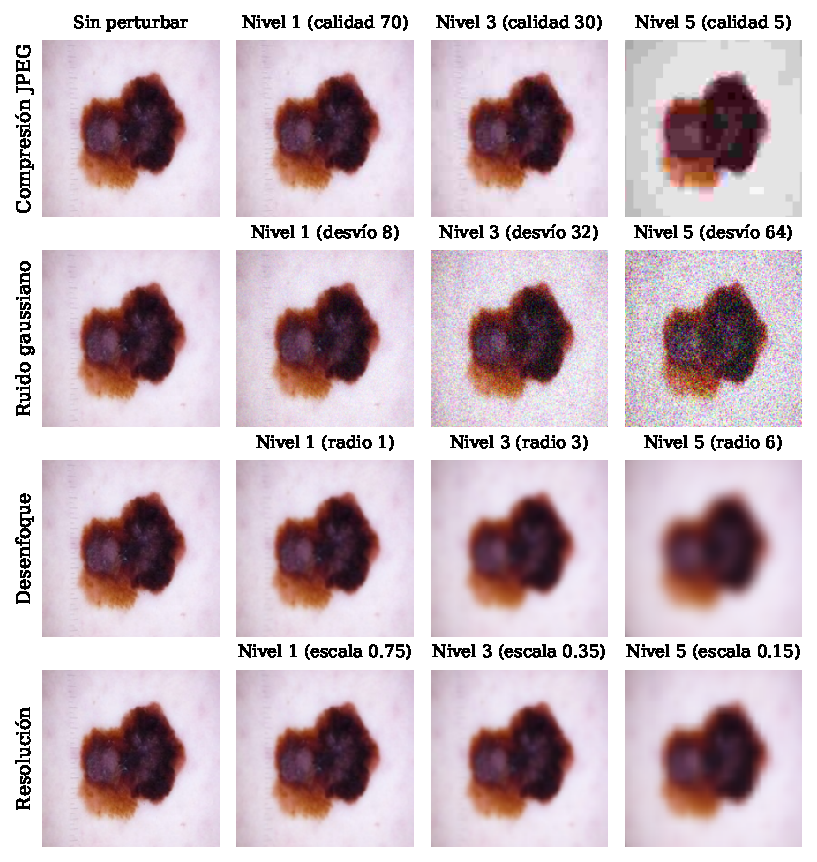
\includegraphics[width=0.72\textwidth]{Figures/Capitulos/03-Materiales-Metodos/perturbaciones-ejemplo.pdf}
    \caption{Una imagen del conjunto de prueba con cada perturbación de la evaluación de robustez, en los niveles 1, 3 y 5.}
    \label{fig:met_perturbaciones}
\end{figure}

\subsection{Calibración}
\label{sec:met_calibracion}

La cuarta evaluación busca saber cuánto se puede confiar en la probabilidad que da el modelo, que fija el umbral de
melanoma y que un clínico leería como certeza. Para ello se miden el ECE y el Brier
(Sección~\ref{sec:marco_eval_calib}) sin calibrar y con dos ajustes posteriores, \emph{temperature scaling} y
\emph{vector scaling}, que se ajustan en validación y se evalúan en el conjunto de prueba. Como el modelo guarda las
probabilidades promediadas con \gls{tta} y no sus salidas previas a la softmax, ambos ajustes se aplican sobre el
logaritmo de esas probabilidades, una aproximación que se declara. Además, dado que los pesos por clase alteran la
confianza del modelo, se comparan dos versiones de la misma configuración, entrenadas con y sin ellos.

\subsection{Interpretabilidad}
\label{sec:met_interpretabilidad}

La quinta evaluación examina en qué parte de la imagen se apoya el modelo. Para ello se aplica Grad-CAM
(Sección~\ref{sec:marco_eval_gradcam}) a Swin-Tiny, sobre la última etapa de la red y para la clase predicha, en siete imágenes de prueba, una por clase, con una sola vista, y en dos errores seleccionados entre los de activación
más alejada del centro de la imagen. Es una inspección cualitativa, que muestra si la activación cae sobre la lesión,
pero no mide el acierto ni respalda un razonamiento clínico.

\subsection{Costo computacional}
\label{sec:met_costo}

La última evaluación estima el costo computacional de ejecutar los modelos y el \emph{pipeline}, que es parte de la
restricción de la Sección~\ref{sec:met_tareas}. Para los clasificadores se miden los parámetros, la memoria máxima en
la GPU, el tiempo por imagen y las imágenes procesadas por segundo. Para los generadores, en cambio, se mide la memoria máxima al generar y se toma el tiempo por reporte de las ejecuciones
de la generación, que comparten instrucción, decodificación y límite de tokens,
de modo que la diferencia refleja el modelo y la longitud de lo que escribe. No es una medición controlada, sino una
estimación del orden de magnitud, que permite contrastar el \emph{pipeline} con el cómputo que usan los trabajos
revisados (Tabla~\ref{tab:marco_brechas} del Capítulo~\ref{cp:marco}). Las condiciones de la medición se detallan en
la Sección~\ref{sec:met_entorno}.

Con estas evaluaciones, quedan definidos todos los experimentos del trabajo, y falta ordenarlos según la parte del
problema que aborda cada uno.

% Extensión estimada: algo más de una página y la tabla de experimentos (ficha 3.9).
% Fuentes: Secciones 3.3 a 3.8 de este capítulo (no agrega experimentos: los ordena por etapas). Ejecuciones por
% configuración: búsqueda con una ejecución por configuración, tres ejecuciones por clasificador supervisado, una por
% función de pérdida; VLM y generadores con decodificación voraz o verosimilitud, deterministas.
% Revisión del tutor del 26/10/2026 (audio 7): la configuración de los experimentos estaba suelta al final de 3.8;
% se ordena por etapas, separando imágenes y reportes, y se dice cuántas ejecuciones tiene cada configuración.
\section{Diseño de los experimentos}
\label{sec:met_diseno}

Las secciones anteriores describen cada componente, el \emph{pipeline} y la forma de evaluarlos. Los experimentos que
los ponen a prueba se organizan por etapas, de modo que cada etapa usa lo que produjo la anterior, y se dividen en dos
partes. La primera parte trabaja con la clasificación de las imágenes y produce el clasificador del
\emph{pipeline}. La segunda trabaja con los reportes y usa ese clasificador como primer componente del
\emph{pipeline}, que solo interviene en esta parte.

La clasificación de las imágenes se evalúa en cuatro etapas:
\begin{enumerate}[leftmargin=1.6em]
    \item \textbf{Búsqueda de hiperparámetros.} Swin-Tiny y ConvNeXt-Tiny se entrenan con las 30 configuraciones de
    la Sección~\ref{sec:met_supervisados_ensamble}, y la validación elige una por modelo.
    \item \textbf{Comparación de los clasificadores supervisados.} Los cuatro modelos se entrenan con la configuración
    elegida, se combinan los dos de la búsqueda en el ensamble y se fija en validación el umbral de melanoma.
    \item \textbf{Variantes y evaluaciones complementarias.} Sobre los modelos de la etapa anterior se comparan las
    funciones de pérdida para el desbalance, se estima el efecto de la fuga de información y se aplican las
    evaluaciones de la Sección~\ref{sec:met_complementarios}.
    \item \textbf{Clasificación con \glspl{vlm}.} Mini-VLM, LLaVA-Med y DermLIP clasifican la misma prueba, sin ajuste y
    con las estrategias y los controles de la Sección~\ref{sec:met_clasif_vlm}, y se comparan con los supervisados.
\end{enumerate}

La generación de reportes, por su parte, avanza en tres etapas, que agregan de a uno los componentes del
\emph{pipeline}:
\begin{enumerate}[leftmargin=1.6em]
    \item \textbf{Generador solo.} Mini-VLM y LLaVA-Med se ajustan sobre \emph{SkinCaRe}
    (Sección~\ref{sec:met_generacion}) y, con SkinVL, generan reportes sin diagnóstico, que se comparan con los textos
    de referencia (Nivel~1) y se evalúan sobre \emph{HAM10000} (Nivel~2).
    \item \textbf{Cascada.} Los tres generadores reciben el diagnóstico de las cuatro fuentes de la
    Sección~\ref{sec:met_referencias}, con las dos variantes que separan la imagen del diagnóstico y con las plantillas
    de recuperación.
    \item \textbf{\emph{Pipeline} completo.} El ruteo por concordancia decide el tipo de reporte de cada caso, y el
    resultado se compara con la cascada y con la línea base sin generador.
\end{enumerate}

El número de ejecuciones depende de si el resultado varía al repetirlo. Cada configuración de la búsqueda y cada
función de pérdida se entrenan una vez, mientras que los cuatro clasificadores supervisados se entrenan tres veces con
la configuración elegida, de modo que sus resultados se informan como media y desvío de las tres ejecuciones
(Sección~\ref{sec:met_seleccion}). Los \glspl{vlm} sin ajuste, las cabezas sobre los \emph{embeddings} y los
generadores, en cambio, se ejecutan una vez por configuración, porque la verosimilitud y la decodificación voraz
devuelven la misma salida para la misma entrada. Cada generador, por su parte, se ajusta una sola vez.

La Tabla~\ref{tab:met_experimentos} reúne los experimentos con lo que busca cada uno, los datos sobre los que se mide y
su métrica principal. El Capítulo~\ref{cp:res_clasif} presenta los resultados de la primera parte, la clasificación
de las imágenes, y el Capítulo~\ref{cp:res_gen}, los de la segunda, la generación de reportes con el
\emph{pipeline}.

\begingroup
\small
\setlength{\tabcolsep}{3pt}
\begin{longtable}{@{}>{\raggedright\arraybackslash}p{3.5cm}
    >{\raggedright\arraybackslash\hspace{0pt}}p{4.3cm}
    >{\raggedright\arraybackslash\hspace{0pt}}p{2.6cm}
    >{\raggedright\arraybackslash\hspace{0pt}}p{3.5cm}@{}}
    \caption{Experimentos del trabajo: qué busca cada uno, sobre qué datos se mide y con qué métrica.}
    \label{tab:met_experimentos}\\
    \toprule
    \textbf{Experimento} & \textbf{Qué se busca} & \textbf{Datos} & \textbf{Métrica principal} \\
    \midrule
    \endfirsthead
    \toprule
    \textbf{Experimento} & \textbf{Qué se busca} & \textbf{Datos} & \textbf{Métrica principal} \\
    \midrule
    \endhead
    \bottomrule
    \endlastfoot
    Clasificadores supervisados (Sección~\ref{sec:met_supervisados})
        & Comparar las dos familias de arquitecturas con el mismo procedimiento
        & Prueba de \emph{HAM10000}
        & Sensibilidad macro; F1 macro \\
    \filasep
    Funciones de pérdida para el desbalance
        & Ver si otra función de pérdida mejora las clases minoritarias
        & Prueba de \emph{HAM10000}
        & Sensibilidad macro \\
    \filasep
    Detección de melanoma
        & Detectar melanomas con un tope de falsas alarmas
        & Prueba de \emph{HAM10000}
        & Sensibilidad y especificidad con umbral; AUC \\
    \filasep
    Fuga de información (Sección~\ref{sec:met_particiones})
        & Estimar cuánto sobreestimaba la fuga el desempeño
        & Prueba completa y subconjunto sin lesiones compartidas
        & Sensibilidad macro \\
    \filasep
    Clasificación con \glspl{vlm} (Sección~\ref{sec:met_clasif_vlm})
        & Saber si un \gls{vlm} clasifica tan bien como un supervisado
        & Prueba de \emph{HAM10000}; fotografías clínicas de \emph{SkinCAP} como control
        & Sensibilidad macro; McNemar con Holm \\
    \filasep
    Generación con referencia
        & Medir el parecido del reporte con un texto de referencia
        & Prueba de \emph{MM-Skin} y de \emph{SkinCoT}
        & Nivel~1 (BLEU-4, ROUGE-L, METEOR, CIDEr, BERTScore) \\
    \filasep
    Ajuste del modelo de lenguaje de Mini-VLM (Sección~\ref{sec:met_generacion})
        & Ver si ajustar también el modelo de lenguaje cambia el reporte
        & Prueba de \emph{HAM10000} y de \emph{SkinCoT}
        & Diferencia pareada de la consistencia diagnóstica; Nivel~1 \\
    \filasep
    Cascada con cuatro fuentes (Sección~\ref{sec:met_referencias})
        & Saber si el reporte afirma el diagnóstico correcto y cuánto aporta el anclaje
        & Prueba de \emph{HAM10000}
        & Consistencia diagnóstica \\
    \filasep
    Cascada sin imagen y con diagnóstico equivocado (Sección~\ref{sec:met_referencias})
        & Separar lo que el reporte toma de la imagen de lo que toma del diagnóstico
        & 400 imágenes de la prueba de \emph{HAM10000}; la prueba completa con SkinVL
        & Consistencia diagnóstica \\
    \filasep
    Recuperación (Sección~\ref{sec:met_recuperacion})
        & Ver si los casos parecidos mejoran el reporte
        & Prueba de \emph{HAM10000}
        & Consistencia diagnóstica \\
    \filasep
    Ruteo en tres niveles (Sección~\ref{sec:met_ruteo})
        & Ver si la concordancia separa aciertos de errores y cuánto aporta el generador
        & Prueba de \emph{HAM10000}
        & Consistencia diagnóstica por nivel; proporción de casos en cada nivel \\
    \filasep
    Generalización (Sección~\ref{sec:met_hiba})
        & Ver si el desempeño se sostiene en otra población
        & \emph{HIBA}
        & Sensibilidad macro \\
    \filasep
    Robustez (Sección~\ref{sec:met_robustez})
        & Medir la caída ante peores condiciones de captura
        & Prueba de \emph{HAM10000} perturbada
        & Caída relativa de la sensibilidad macro \\
    \filasep
    Calibración (Sección~\ref{sec:met_calibracion})
        & Saber cuánto se puede confiar en la probabilidad
        & Validación y prueba de \emph{HAM10000}
        & ECE; Brier \\
    \filasep
    Interpretabilidad (Sección~\ref{sec:met_interpretabilidad})
        & Ver en qué parte de la imagen se apoya el modelo
        & Siete imágenes de prueba
        & Inspección cualitativa \\
    \filasep
    Costo computacional (Sección~\ref{sec:met_costo})
        & Estimar el costo de ejecutar los modelos y el \emph{pipeline}
        & Prueba de \emph{HAM10000}
        & Parámetros; tiempo por imagen y por reporte \\
\end{longtable}
\endgroup

% Extensión estimada: algo más de media página, tres párrafos.
% Fuentes: Codigo/CLAUDE.md (GPU de cada clúster y del equipo local, bf16 en Ampere o posterior);
% Codigo/requirements.txt y src/models/{classifiers,dermlip,mini_vlm}.py (bibliotecas); scripts/measure_cost.py
% (costo de los clasificadores en la RTX 4070, lotes de 32); Apéndice E (ap:reproducibilidad).
% Revisión del tutor del 21/10/2026: sección nueva que reúne el hardware, las semillas y las bibliotecas, antes
% dispersos en 3.1, 3.3, 3.6 y 3.8. Sin versiones de CUDA ni herramientas internas (regla R1 del autor).
\section{Entorno experimental y recursos computacionales}
\label{sec:met_entorno}

Los experimentos se ejecutaron en tres GPU, todas dentro de la restricción de la Sección~\ref{sec:met_tareas}. Los
clasificadores supervisados se entrenaron en una RTX 4080 de 16~GB, en el clúster TOKO de la Universidad Nacional de
Cuyo. El ajuste de los \glspl{vlm} y la generación de los reportes se ejecutaron en una A30 de 24~GB, en el clúster
Mendieta de la Universidad Nacional de Córdoba. La A30 es una GPU de centro de datos, pero tiene la misma memoria que
una de consumo de gama alta, que es lo que fija la restricción. Por último, una RTX 4070 de 12~GB, en un equipo personal, se usó para
calcular las métricas de generación y para medir el costo de los clasificadores. Las tres GPU tienen arquitectura Ampere
o posterior, lo que permite entrenar en precisión \emph{bfloat16} (bf16) en todos los casos.

En cuanto a la medición del costo (Sección~\ref{sec:met_costo}), el tiempo de inferencia, la cantidad de imágenes por
segundo y la memoria máxima de los clasificadores se midieron en la RTX 4070, con una imagen y con lotes de 32, en la
misma precisión bf16 con que se evalúan. El tiempo por reporte de los
generadores, en cambio, se tomó de las ejecuciones de la generación en la A30. Como las dos mediciones se hicieron en
GPU distintas, la comparación entre clasificadores y generadores es solo de orden de magnitud.

El código usa PyTorch y torchvision para los clasificadores supervisados, las bibliotecas \texttt{transformers} y
\texttt{peft} de Hugging Face para los \glspl{vlm} generativos y LoRA, \texttt{open\_clip} para DermLIP y scikit-learn
para las cabezas clásicas, la partición y las métricas. Todos los entrenamientos fijan la semilla 42, que es
también la de la ejecución que usan las pruebas y el \emph{pipeline}, y las otras dos ejecuciones de cada
clasificador supervisado (Sección~\ref{sec:met_supervisados_ensamble}) usan las semillas 43 y 44. El
Apéndice~\ref{ap:reproducibilidad} reúne lo necesario para repetir cada experimento.

